\section{Auswertung}
Aus den aufgenommenen Messreihen für den Relaxationsstrom bei zwei verschiedenen Heizraten soll
nun die Aktivierungsenergie $W$ sowie die Relaxationszeit $\tau$ bestimmt werden. Die Aktivierungsenergie
wird dabei auf zwei verschiedene Weisen bestimmt, zum einen aus der Anlaufkurve und zum anderen
durch Integration. Da der Relaxationsstrom und die Relaxationsstromdichte sich nur durch einen
konstanten Faktor unterscheiden, können die zuvor gegebenen Relationen für die Relaxationsstromdichte
verwendet werden.

\subsection{Auswertung der 1. Heizrate}
Zunächst wird aus den Messwerten im Anhang die mittlere Heizrate bestimmt, welche
sich zu
\begin{equation}
  b_1=\SI{1,99(5)}{\K\per\min}
\end{equation}
ergibt.
Um die Aktivierungsenergie durch eine lineare Ausgleichsrechnung zu bestimmen, wird zunächst
der Relaxationsstrom gegen die Temperatur aufgetragen. Dies ist in Abbildung \ref{fig:Fig1}
dargestellt. Da das erste Maximum des Relaxationsstroms,
welches im Folgenden genauer untersucht wird, auf der steigenden Flanke des zweiten Maximums
liegt, wird dieser "Untergrund" von den Messwerten abgezogen. Dazu wird eine Regression der
Form
\begin{equation}
  f(T)=a\cdot\exp(-b/T)
\end{equation}
durchgeführt, wobei hierfür nur die in Abbildung \ref{fig:Fig1} mit * markierten Messwerte verwendet werden.
Die um den Untergrund bereinigten Messwerte sind in Abbildung \ref{fig:Fig2} dargestellt. Dabei sind die
verwendeten Messwerte für die Berechnung der Aktivierungsenergie über den Anlaufstrom in schwarz dargestellt.
Für die Berechnung mittels des Integrals werden die schwarz und blau markierten Messwerte verwendet.

\begin{figure}[H]
  \centering
  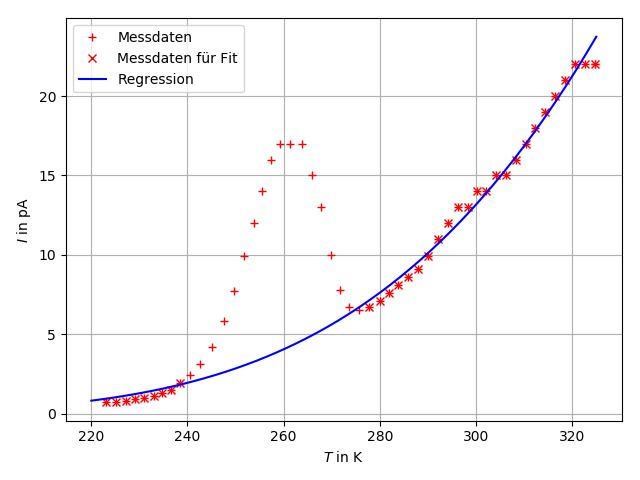
\includegraphics[width=0.75\textwidth]{Dipol1mitUntergrund.png}
  \caption{In rot sind die Messwerte des Relaxationsstroms gegen die Temperatur aufgetragen. Die in
  blau eingezeichnete Regression für den Untergrund wird aus den mit * gekennzeichneten
  Werten berechnet.}
  \label{fig:Fig1}
\end{figure}

\begin{figure}[H]
  \centering
  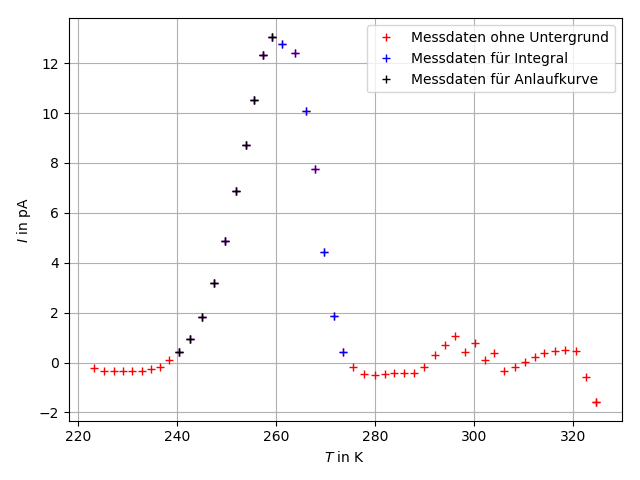
\includegraphics[width=0.75\textwidth]{Dipol1ohneUntergrund.png}
  \caption{Die um den Untergrund bereinigten Messwerte des Relaxationsstroms aufgetragen gegen die
  Temperatur. Zusätzlich ist farblich markiert, welche Messwerte für die Weiteren Berechnungen der Aktivierungsenergie
  verwendet werden.}
  \label{fig:Fig2}
\end{figure}


\textbf{Aktivierungsenergie aus der Anlaufkurve}\\
Zur Bestimmung der Aktivierungsenergie $W$ werden die in Abbildung \ref{fig:Fig2} schwarz
markierten Messwerte verwendet. Diese können durch die Formel \ref{eqn:stromnäherung} genähert werden,
welche logarithmisch gegen $\sfrac{1}{T}$ aufgetragen einer Geraden entsprechen. Mit einer
Ausgleichsgeraden der Form
\begin{equation}
  f(T)=m\cdot x+b
\end{equation}
ergeben sich die Parameter
\begin{align*}
  |m|&=\SI{11100(900)}{}\;\; \text{und}\\
  b&=\SI{46(4)}{}.
\end{align*}
Das zugehörige Diagramm mit den logarithmierten Messwerte und der Ausgleichsgerade ist in Diagramm \ref{fig:Fig3}
dargestellt.

\begin{figure}
  \centering
  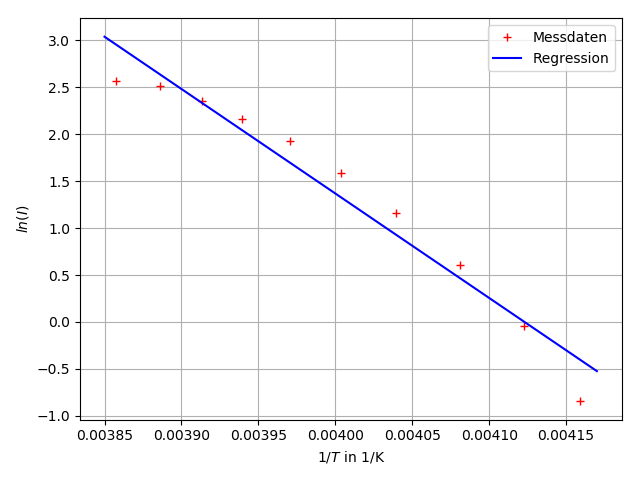
\includegraphics[width=0.75\textwidth]{Dipol1Anlauf.png}
  \caption{Messwerte der Anlaufkurve, welche logarithmiert gegen $\sfrac{1}{T}$ aufgetragen und mit
  einer linearen Regression gefittet werden.}
  \label{fig:Fig3}
\end{figure}

Aus den so erhaltenen Parametern lässt sich über
\begin{equation}
  W=k_{B}\cdot |m|
  \label{eqn:Aktivierung}
\end{equation}
die Aktivierungsenergie $W$ aus der Steigung der Ausgleichsgeraden zu $W_\text{A,1}=\SI{0,96(8)}{\eV}$ bestimmen.
\\
\\
\textbf{Aktivierungsenergie durch Integration}\\
Um die Aktivierungsenergie durch Integrieren zu bestimmen, werden sowohl die schwarz als auch blau markierten
Werte aus Diagramm \ref{fig:Fig2} verwendet. Unter Verwendung von Gleichung \ref{eqn:integral} ergibt sich aufgetragen
gegen $\sfrac{1}{T}$ ein nahezu linearer Verlauf, welcher erneut mit einer linearen Ausgleichsgerade der
Form $f(T)=m\cdot x+b$ angenähert werden kann. Die Ausgleichsrechnung liefert die Parameter
\begin{align}
  |m|&=\SI{12000(400)}{}\;\; \text{und}\\
  b&=\SI{44(2)}{}.
\end{align}

\begin{figure}[H]
  \centering
  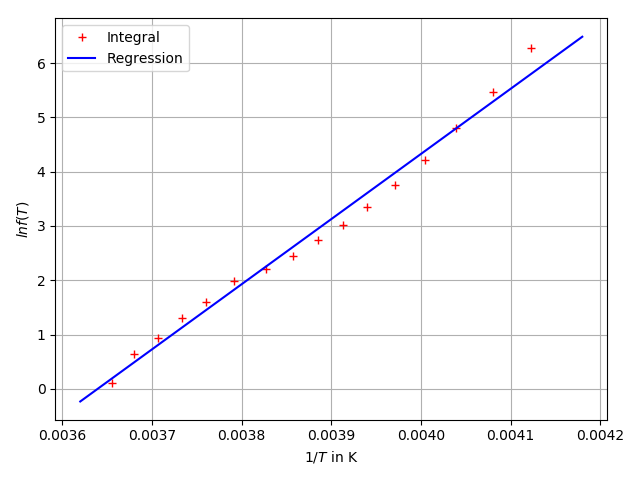
\includegraphics[width=0.75\textwidth]{Dipol1Integral.png}
  \caption{Die nach Formel \ref{eqn:integral} aus den Messwerten berechneten Werte aufgetragen
  gegen $\sfrac{1}{T}$ und mit einer linearen Regression gefittet.}
  \label{fig:Fig4}
\end{figure}

Für die Aktivierungsenergie folgt daraus $W_\text{I,1}=\SI{1,03(4)}{\eV}$.

\subsection{Auswertung der 2. Heizrate}
Die Auswertung für die zweite Heizrate, dessen Mittelwert sich zu
\begin{equation}
  b_2=\SI{1,06(2)}{\K\per\min}
\end{equation}
bestimmen lässt, erfolgt völlig analog zur Auswertung der ersten Heizrate.
Der gemessene Relaxationsstrom sowie die Regression sind in Diagramm \ref{fig:Abb1} dargestellt, während
die um den Untergrund bereinigten Werte in Diagramm \ref{fig:Abb2} zu sehen sind. Erneut sind die Messwerte, welche für
die Berechnung der Aktivierungsenergie über den Anlaufstrom verwendet wurden schwarz markiert. Für die Berechnung
mithilfe des Integrals werden wieder die schwarz und blau markierten Werte verwendet.

\begin{figure}
  \centering
  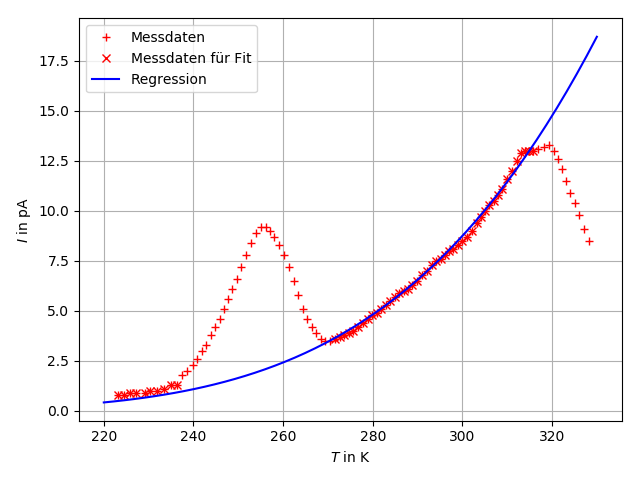
\includegraphics[width=0.75\textwidth]{Dipol2mitUntergrund.png}
  \caption{In rot sind die Messwerte des Relaxationsstroms gegen die Temperatur aufgetragen. Die in
  blau eingezeichnete Regression für den Untergrund wird aus den mit * gekennzeichneten
  Werten berechnet.}
  \label{fig:Abb1}
\end{figure}

\begin{figure}[H]
  \centering
  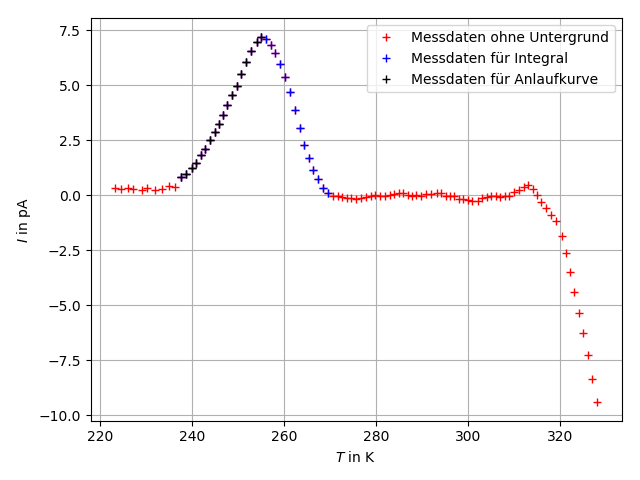
\includegraphics[width=0.75\textwidth]{Dipol2ohneUntergrund.png}
  \caption{Die um den Untergrund bereinigten Messwerte des Relaxationsstroms aufgetragen gegen die
  Temperatur. Zusätzlich ist farblich markiert, welche Messwerte für die Weiteren Berechnungen der Aktivierungsenergie
  verwendet werden.}
  \label{fig:Abb2}
\end{figure}


\textbf{Aktivierungsenergie aus der Anlaufkurve}\\
Die lineare Ausgleichsrechnung aus der Anlaufkurve liefert die Werte
\begin{align*}
  |m|&=\SI{7700(310)}{}\;\; \text{und}\\
  b&=\SI{32,3(13)}{}
\end{align*}
woraus sich nach Formel \ref{eqn:Aktivierung} die Aktivierungsenergie $W_\text{A,2}=\SI{0,66(3)}{\eV}$
bestimmen lässt.

\begin{figure}[H]
  \centering
  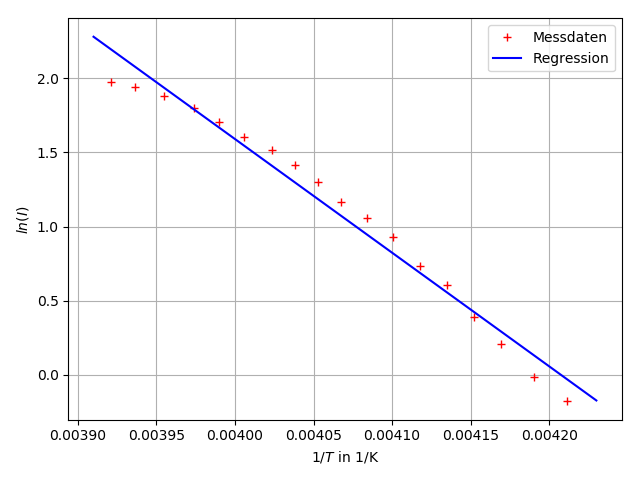
\includegraphics[width=0.75\textwidth]{Dipol2Anlauf.png}
  \caption{Messwerte der Anlaufkurve, welche logarithmiert gegen $\sfrac{1}{T}$ aufgetragen und mit
  einer linearen Regression gefittet werden.}
  \label{fig:Abb3}
\end{figure}

\textbf{Aktivierungsenergie durch Integration}\\
Aus der linearen Ausgleichsrechnung der integrierten Werte, welche in Diagramm \ref{fig:Abb4}
zu sehen ist, ergeben sich die Parameter
\begin{align}
  |m|&=\SI{10100(200)}{}\;\; \text{und}\\
  b&=\SI{37(1)}{}.
\end{align}
Daraus ergibt sich eine Aktivierungsenergie von $W_\text{I,2}=\SI{0,87(2)}{\eV}$

\begin{figure}[H]
  \centering
  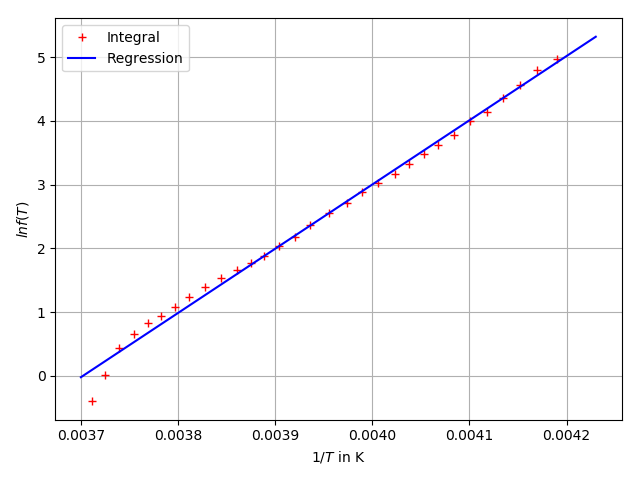
\includegraphics[width=0.75\textwidth]{Dipol2Integral.png}
  \caption{Die nach Formel \ref{eqn:integral} aus den Messwerten berechneten Werte aufgetragen
  gegen $\sfrac{1}{T}$ und mit einer linearen Regression gefittet.}
  \label{fig:Abb4}
\end{figure}

\subsection{Bestimmung der charakteristischen Relaxationszeit}
Mittels Gleichung \ref{eqn:taumax} lässt sich zunächst $\tau_\text{max}$ bestimmen. Dazu
werden aus den Diagrammen \ref{fig:Fig2} und \ref{fig:Abb2} die Temperaturen bestimmt, an den $I$ maximal ist:
\begin{align*}
  T_\text{max1}&=\SI{259,25}{\K}\;\;\text{und}\\
  T_\text{max2}&=\SI{255,05}{\K}.
\end{align*}

Unter Verwendung der berechneten Aktivierungsenergien ergeben sich mittels Gleichung \ref{eqn:taumax}
folgende Werte für $\tau_\text{max}$:
\begin{align*}
\tau_\text{max1,A}&=\SI{3.03(25)}{\s}\;\;\;&\tau_\text{max2,A}&=\SI{7.99(35)}{\s}\\
\tau_\text{max1,I}&=\SI{2.81(11)}{\s}\;\;\;&\tau_\text{max2,I}&=\SI{6.09(14)}{\s}.
\end{align*}

Eingesetzt in Gleichung \ref{eqn:tau} ergeben sich daraus die Werte für
die charakteristische Relaxationszeit $\tau_0$:

\begin{align*}
\tau_\text{01,A}&=\SI{0.7(24)e-18}{\s}\;\;\;&\tau_\text{02,A}&=\SI{7(8)e-13}{\s}\\
\tau_\text{01,I}&=\SI{4(5)e-20}{\s}\;\;\;&\tau_\text{02,I}&=\SI{9(5)e-17}{\s}.
\end{align*}

Dabei wird der Fehler von $\tau_0$ mit der Gauß´schen Fehlerfortpflanzung:
\begin{equation}
  \delta f = \sqrt{ \sum_{i=1}^N \left( \frac{\partial f}{\partial x_i}\right)^2
  \cdot (\delta x_i)^2  } \:
  \label{eqn:gaus}
\end{equation}
berechnet, welche sich für diesen Fall zu
\begin{equation}
  \Delta \tau_0= \sqrt{\Bigg(\exp\Big(\frac{-W}{k_B T}\Big)\cdot\Delta\tau_\text{max}\Bigg)^2\cdot\Bigg(\tau_\text{max}\cdot\exp\Big(\frac{-W}{k_B T}\Big)\Big(\frac{-\Delta W}{k_B T}\Big)  \Bigg)^2}
\end{equation}
ergibt.
